% Options for packages loaded elsewhere
\PassOptionsToPackage{unicode}{hyperref}
\PassOptionsToPackage{hyphens}{url}
%
\documentclass[
]{book}
\usepackage{amsmath,amssymb}
\usepackage{iftex}
\ifPDFTeX
  \usepackage[T1]{fontenc}
  \usepackage[utf8]{inputenc}
  \usepackage{textcomp} % provide euro and other symbols
\else % if luatex or xetex
  \usepackage{unicode-math} % this also loads fontspec
  \defaultfontfeatures{Scale=MatchLowercase}
  \defaultfontfeatures[\rmfamily]{Ligatures=TeX,Scale=1}
\fi
\usepackage{lmodern}
\ifPDFTeX\else
  % xetex/luatex font selection
\fi
% Use upquote if available, for straight quotes in verbatim environments
\IfFileExists{upquote.sty}{\usepackage{upquote}}{}
\IfFileExists{microtype.sty}{% use microtype if available
  \usepackage[]{microtype}
  \UseMicrotypeSet[protrusion]{basicmath} % disable protrusion for tt fonts
}{}
\makeatletter
\@ifundefined{KOMAClassName}{% if non-KOMA class
  \IfFileExists{parskip.sty}{%
    \usepackage{parskip}
  }{% else
    \setlength{\parindent}{0pt}
    \setlength{\parskip}{6pt plus 2pt minus 1pt}}
}{% if KOMA class
  \KOMAoptions{parskip=half}}
\makeatother
\usepackage{xcolor}
\usepackage{color}
\usepackage{fancyvrb}
\newcommand{\VerbBar}{|}
\newcommand{\VERB}{\Verb[commandchars=\\\{\}]}
\DefineVerbatimEnvironment{Highlighting}{Verbatim}{commandchars=\\\{\}}
% Add ',fontsize=\small' for more characters per line
\usepackage{framed}
\definecolor{shadecolor}{RGB}{248,248,248}
\newenvironment{Shaded}{\begin{snugshade}}{\end{snugshade}}
\newcommand{\AlertTok}[1]{\textcolor[rgb]{0.94,0.16,0.16}{#1}}
\newcommand{\AnnotationTok}[1]{\textcolor[rgb]{0.56,0.35,0.01}{\textbf{\textit{#1}}}}
\newcommand{\AttributeTok}[1]{\textcolor[rgb]{0.13,0.29,0.53}{#1}}
\newcommand{\BaseNTok}[1]{\textcolor[rgb]{0.00,0.00,0.81}{#1}}
\newcommand{\BuiltInTok}[1]{#1}
\newcommand{\CharTok}[1]{\textcolor[rgb]{0.31,0.60,0.02}{#1}}
\newcommand{\CommentTok}[1]{\textcolor[rgb]{0.56,0.35,0.01}{\textit{#1}}}
\newcommand{\CommentVarTok}[1]{\textcolor[rgb]{0.56,0.35,0.01}{\textbf{\textit{#1}}}}
\newcommand{\ConstantTok}[1]{\textcolor[rgb]{0.56,0.35,0.01}{#1}}
\newcommand{\ControlFlowTok}[1]{\textcolor[rgb]{0.13,0.29,0.53}{\textbf{#1}}}
\newcommand{\DataTypeTok}[1]{\textcolor[rgb]{0.13,0.29,0.53}{#1}}
\newcommand{\DecValTok}[1]{\textcolor[rgb]{0.00,0.00,0.81}{#1}}
\newcommand{\DocumentationTok}[1]{\textcolor[rgb]{0.56,0.35,0.01}{\textbf{\textit{#1}}}}
\newcommand{\ErrorTok}[1]{\textcolor[rgb]{0.64,0.00,0.00}{\textbf{#1}}}
\newcommand{\ExtensionTok}[1]{#1}
\newcommand{\FloatTok}[1]{\textcolor[rgb]{0.00,0.00,0.81}{#1}}
\newcommand{\FunctionTok}[1]{\textcolor[rgb]{0.13,0.29,0.53}{\textbf{#1}}}
\newcommand{\ImportTok}[1]{#1}
\newcommand{\InformationTok}[1]{\textcolor[rgb]{0.56,0.35,0.01}{\textbf{\textit{#1}}}}
\newcommand{\KeywordTok}[1]{\textcolor[rgb]{0.13,0.29,0.53}{\textbf{#1}}}
\newcommand{\NormalTok}[1]{#1}
\newcommand{\OperatorTok}[1]{\textcolor[rgb]{0.81,0.36,0.00}{\textbf{#1}}}
\newcommand{\OtherTok}[1]{\textcolor[rgb]{0.56,0.35,0.01}{#1}}
\newcommand{\PreprocessorTok}[1]{\textcolor[rgb]{0.56,0.35,0.01}{\textit{#1}}}
\newcommand{\RegionMarkerTok}[1]{#1}
\newcommand{\SpecialCharTok}[1]{\textcolor[rgb]{0.81,0.36,0.00}{\textbf{#1}}}
\newcommand{\SpecialStringTok}[1]{\textcolor[rgb]{0.31,0.60,0.02}{#1}}
\newcommand{\StringTok}[1]{\textcolor[rgb]{0.31,0.60,0.02}{#1}}
\newcommand{\VariableTok}[1]{\textcolor[rgb]{0.00,0.00,0.00}{#1}}
\newcommand{\VerbatimStringTok}[1]{\textcolor[rgb]{0.31,0.60,0.02}{#1}}
\newcommand{\WarningTok}[1]{\textcolor[rgb]{0.56,0.35,0.01}{\textbf{\textit{#1}}}}
\usepackage{longtable,booktabs,array}
\usepackage{calc} % for calculating minipage widths
% Correct order of tables after \paragraph or \subparagraph
\usepackage{etoolbox}
\makeatletter
\patchcmd\longtable{\par}{\if@noskipsec\mbox{}\fi\par}{}{}
\makeatother
% Allow footnotes in longtable head/foot
\IfFileExists{footnotehyper.sty}{\usepackage{footnotehyper}}{\usepackage{footnote}}
\makesavenoteenv{longtable}
\usepackage{graphicx}
\makeatletter
\def\maxwidth{\ifdim\Gin@nat@width>\linewidth\linewidth\else\Gin@nat@width\fi}
\def\maxheight{\ifdim\Gin@nat@height>\textheight\textheight\else\Gin@nat@height\fi}
\makeatother
% Scale images if necessary, so that they will not overflow the page
% margins by default, and it is still possible to overwrite the defaults
% using explicit options in \includegraphics[width, height, ...]{}
\setkeys{Gin}{width=\maxwidth,height=\maxheight,keepaspectratio}
% Set default figure placement to htbp
\makeatletter
\def\fps@figure{htbp}
\makeatother
\setlength{\emergencystretch}{3em} % prevent overfull lines
\providecommand{\tightlist}{%
  \setlength{\itemsep}{0pt}\setlength{\parskip}{0pt}}
\setcounter{secnumdepth}{5}
\usepackage{booktabs}
\ifLuaTeX
  \usepackage{selnolig}  % disable illegal ligatures
\fi
\usepackage[]{natbib}
\bibliographystyle{apalike}
\IfFileExists{bookmark.sty}{\usepackage{bookmark}}{\usepackage{hyperref}}
\IfFileExists{xurl.sty}{\usepackage{xurl}}{} % add URL line breaks if available
\urlstyle{same}
\hypersetup{
  pdftitle={R Projects for Math 3080},
  pdfauthor={Alvaro Arias},
  hidelinks,
  pdfcreator={LaTeX via pandoc}}

\title{R Projects for Math 3080}
\author{Alvaro Arias}
\date{2024-01-22}

\usepackage{amsthm}
\newtheorem{theorem}{Theorem}[chapter]
\newtheorem{lemma}{Lemma}[chapter]
\newtheorem{corollary}{Corollary}[chapter]
\newtheorem{proposition}{Proposition}[chapter]
\newtheorem{conjecture}{Conjecture}[chapter]
\theoremstyle{definition}
\newtheorem{definition}{Definition}[chapter]
\theoremstyle{definition}
\newtheorem{example}{Example}[chapter]
\theoremstyle{definition}
\newtheorem{exercise}{Exercise}[chapter]
\theoremstyle{definition}
\newtheorem{hypothesis}{Hypothesis}[chapter]
\theoremstyle{remark}
\newtheorem*{remark}{Remark}
\newtheorem*{solution}{Solution}
\begin{document}
\maketitle

{
\setcounter{tocdepth}{1}
\tableofcontents
}
\hypertarget{introduction-to-r}{%
\chapter{Introduction to R}\label{introduction-to-r}}

We start reviewing fundamental concepts of the R language.
We assume that you have downloaded and installed RStudio.

Base R refers to the core functionality and built-in functions of the R programming language without any additional packages or libraries. It provides essential data structures (vectors, matrices, data frames, lists), control structures (loops, conditionals), and basic statistical functions.

Libraries, or packages, in R are extensions that add specialized functions and capabilities beyond what's available in base R. They are developed by the R community to address specific tasks or domains. These libraries enhance R's functionality and make it a powerful tool for a wide range of data analysis and statistical tasks.

\hypertarget{variables-and-data-types}{%
\section{Variables and Data Types}\label{variables-and-data-types}}

In R, variables store data and are assigned using \texttt{\textless{}-}. There are various types, including numeric (real or complex numbers), character (strings, written between quotes), and logical or boolean (TRUE or FALSE)

\begin{Shaded}
\begin{Highlighting}[]
\NormalTok{x }\OtherTok{\textless{}{-}} \DecValTok{2}
\NormalTok{y }\OtherTok{\textless{}{-}} \StringTok{"I am a string"}
\NormalTok{z }\OtherTok{\textless{}{-}} \ConstantTok{TRUE}

\FunctionTok{print}\NormalTok{(x)}
\CommentTok{\#\textgreater{} [1] 2}
\FunctionTok{print}\NormalTok{(y)}
\CommentTok{\#\textgreater{} [1] "I am a string"}
\FunctionTok{print}\NormalTok{(z)}
\CommentTok{\#\textgreater{} [1] TRUE}
\end{Highlighting}
\end{Shaded}

\hypertarget{logical-operators-and-conditionals}{%
\section{Logical Operators and Conditionals}\label{logical-operators-and-conditionals}}

The logical operators perform logical operations on boolean values. They include:

\begin{itemize}
\tightlist
\item
  AND that is represented by \(\wedge\) in logic and by \texttt{\&} in R.
\item
  OR that is represented by \(\vee\) in logic and by \texttt{\textbar{}} in R.
\item
  NOT that is represented by \(\neg\) in logic and by \texttt{!} in R.
\end{itemize}

AND and OR are formally defined by the truth tables below. Note that AND is TRUE only when both values are true, and OR is TRUE when at least one value is true.

\begin{longtable}[]{@{}llll@{}}
\toprule\noalign{}
\(p\) & \(q\) & \(p\wedge q\) & \(p\vee q\) \\
\midrule\noalign{}
\endhead
\bottomrule\noalign{}
\endlastfoot
TRUE & TRUE & TRUE & TRUE \\
TRUE & FALSE & FALSE & TRUE \\
FALSE & TRUE & FALSE & TRUE \\
FALSE & FALSE & FALSE & FALSE \\
\end{longtable}

NOT is defined in the obvious way: \(\neg p\) is FALSE if \(p\) is TRUE and it is TRUE if \(p\) is FALSE.

In R, \texttt{==} is used to check if the objects are equal and \texttt{!=} is used to check if the objects aren't equal. For example, \texttt{1==2} is FALSE and \texttt{1!=2} is TRUE. The comparison symbols \texttt{\textless{}} and \texttt{\textgreater{}} have the same meaning we use in math. Less than or equal \(\leq\) is \texttt{\textless{}=} and greater than or equal \(\geq\) is \texttt{\textgreater{}=}.

Conditionals in R are structures that allow us to execute different blocks of code based on specified conditions. The main conditional statement is the \textbf{if statement}, which can be extended to an \textbf{if else statement} and \textbf{else if clauses}. They have the following syntax:

\begin{verbatim}
if (condition) {
  # Code to execute when the condition is TRUE
}
\end{verbatim}

\begin{verbatim}
if (condition) {
  # Code to execute when the condition is TRUE
} else {
  # Code to execute when the condition is FALSE
}
\end{verbatim}

\begin{verbatim}
if (condition1) {
  # Code to execute when condition1 is TRUE
} else if (condition2) {
  # Code to execute when condition1 is FALSE and condition2 is TRUE
} else {
  # Code to execute when both condition1 and condition2 are FALSE
}
\end{verbatim}

\hypertarget{functions}{%
\section{Functions}\label{functions}}

The functions in R have the following syntax:

\begin{verbatim}
function_name <- function(arg1, arg2, ...) {
  # Code defining the function's behavior
  return(result)
}
\end{verbatim}

The functions \(f\) and \(g\) below demonstrate simple examples. The function \(g\) also illustrates the use of conditionals.

\[f(x)=2x^2-3x-1\]
\[g(x)=\begin{cases}2x+1&\text{if }x<0\\x^2 &\text{otherwise} \end{cases}\]

\begin{Shaded}
\begin{Highlighting}[]
\NormalTok{f }\OtherTok{\textless{}{-}} \ControlFlowTok{function}\NormalTok{(x)\{}
  \FunctionTok{return}\NormalTok{(}\DecValTok{2}\SpecialCharTok{*}\NormalTok{x}\SpecialCharTok{\^{}}\DecValTok{2{-}3}\SpecialCharTok{*}\NormalTok{x}\DecValTok{{-}1}\NormalTok{)}
\NormalTok{\}}

\NormalTok{g }\OtherTok{\textless{}{-}} \ControlFlowTok{function}\NormalTok{(x) \{}
  \ControlFlowTok{if}\NormalTok{ (x }\SpecialCharTok{\textless{}} \DecValTok{0}\NormalTok{) \{}
\NormalTok{    result }\OtherTok{\textless{}{-}} \DecValTok{2} \SpecialCharTok{*}\NormalTok{ x}\SpecialCharTok{+}\DecValTok{1}
\NormalTok{  \} }\ControlFlowTok{else}\NormalTok{ \{}
\NormalTok{    result }\OtherTok{\textless{}{-}}\NormalTok{ x}\SpecialCharTok{\^{}}\DecValTok{2}
\NormalTok{  \}}
  \FunctionTok{return}\NormalTok{(result)}
\NormalTok{\}}
\end{Highlighting}
\end{Shaded}

We can evaluate the functions.

\begin{Shaded}
\begin{Highlighting}[]
\FunctionTok{f}\NormalTok{(}\DecValTok{0}\NormalTok{)}
\CommentTok{\#\textgreater{} [1] {-}1}
\FunctionTok{g}\NormalTok{(}\SpecialCharTok{{-}}\DecValTok{2}\NormalTok{)}
\CommentTok{\#\textgreater{} [1] {-}3}
\end{Highlighting}
\end{Shaded}

\hypertarget{vectors-and-operations}{%
\section{Vectors and Operations}\label{vectors-and-operations}}

Vectors are fundamental data structures in R that provide a flexible way to work with and manipulate sequences of values.

In R, vectors are one-dimensional arrays that store elements of the \emph{same data type}. Vectors are often created using the \texttt{c(\ )} function and they can be used to represent situations, like a box with 3 red balls, 2 yellow ones and 1 green.

\begin{Shaded}
\begin{Highlighting}[]
\NormalTok{numeric\_vector }\OtherTok{\textless{}{-}} \FunctionTok{c}\NormalTok{(}\DecValTok{1}\NormalTok{,}\DecValTok{2}\NormalTok{,}\DecValTok{3}\NormalTok{,}\DecValTok{4}\NormalTok{,}\DecValTok{5}\NormalTok{)}
\NormalTok{box }\OtherTok{\textless{}{-}} \FunctionTok{c}\NormalTok{(}\StringTok{"red"}\NormalTok{,}\StringTok{"red"}\NormalTok{,}\StringTok{"red"}\NormalTok{,}\StringTok{"yellow"}\NormalTok{,}\StringTok{"yellow"}\NormalTok{,}\StringTok{"green"}\NormalTok{)}
\end{Highlighting}
\end{Shaded}

The \textbf{\emph{colon}} operator \texttt{:} is used to create sequences of numbers with steps of length 1 or -1. The basic syntax is \texttt{start:end}. Here are a few examples:

\begin{Shaded}
\begin{Highlighting}[]
\DecValTok{1}\SpecialCharTok{:}\DecValTok{10}
\CommentTok{\#\textgreater{}  [1]  1  2  3  4  5  6  7  8  9 10}
\DecValTok{20}\SpecialCharTok{:}\DecValTok{12}
\CommentTok{\#\textgreater{} [1] 20 19 18 17 16 15 14 13 12}
\DecValTok{3}\SpecialCharTok{:}\DecValTok{8}
\CommentTok{\#\textgreater{} [1] 3 4 5 6 7 8}
\end{Highlighting}
\end{Shaded}

\hypertarget{indexing-and-subsets}{%
\section{Indexing and Subsets}\label{indexing-and-subsets}}

Elements in a vector are accessed using square brackets and indices. \textbf{\emph{Indexing starts at 1 in R,}} which is different from most programming languages, where indexing typically starts at 0.

\begin{Shaded}
\begin{Highlighting}[]
\NormalTok{x }\OtherTok{\textless{}{-}}\NormalTok{ box[}\DecValTok{3}\NormalTok{]}
\NormalTok{x}
\CommentTok{\#\textgreater{} [1] "red"}
\end{Highlighting}
\end{Shaded}

We can also select a subset of elements using index vectors or boolean vectors.

\begin{Shaded}
\begin{Highlighting}[]
\NormalTok{box[}\DecValTok{2}\SpecialCharTok{:}\DecValTok{4}\NormalTok{]}
\CommentTok{\#\textgreater{} [1] "red"    "red"    "yellow"}
\NormalTok{box[}\FunctionTok{c}\NormalTok{(}\DecValTok{3}\NormalTok{,}\DecValTok{4}\NormalTok{,}\DecValTok{6}\NormalTok{)]}
\CommentTok{\#\textgreater{} [1] "red"    "yellow" "green"}
\NormalTok{numbers }\OtherTok{\textless{}{-}} \DecValTok{1}\SpecialCharTok{:}\DecValTok{6}
\NormalTok{numbers[}\FunctionTok{c}\NormalTok{(T,F,T,F,T,F)]}
\CommentTok{\#\textgreater{} [1] 1 3 5}
\end{Highlighting}
\end{Shaded}

\hypertarget{vectorized-operations}{%
\section{Vectorized Operations}\label{vectorized-operations}}

R supports \emph{vectorized operations}, allowing us to perform operations on entire vectors without the need for explicit loops. Recall that \texttt{numeric\_vector\ \textless{}-\ c(1,2,3,4,5)}.

\begin{Shaded}
\begin{Highlighting}[]
\NormalTok{numeric\_vector}\SpecialCharTok{*}\NormalTok{(}\SpecialCharTok{{-}}\DecValTok{3}\NormalTok{)}
\CommentTok{\#\textgreater{} [1]  {-}3  {-}6  {-}9 {-}12 {-}15}
\NormalTok{numeric\_vector}\SpecialCharTok{\^{}}\DecValTok{3}
\CommentTok{\#\textgreater{} [1]   1   8  27  64 125}
\NormalTok{numeric\_vector}\SpecialCharTok{+}\NormalTok{numeric\_vector}
\CommentTok{\#\textgreater{} [1]  2  4  6  8 10}
\end{Highlighting}
\end{Shaded}

Vectorized operation also supports logical operations

\begin{Shaded}
\begin{Highlighting}[]
\NormalTok{numeric\_vector}\SpecialCharTok{\textgreater{}}\DecValTok{2}
\CommentTok{\#\textgreater{} [1] FALSE FALSE  TRUE  TRUE  TRUE}
\NormalTok{box }\SpecialCharTok{==} \StringTok{"yellow"}
\CommentTok{\#\textgreater{} [1] FALSE FALSE FALSE  TRUE  TRUE FALSE}
\end{Highlighting}
\end{Shaded}

We can combine these features to select objects satisfying certain properties

\begin{example}
Suppose that \texttt{x\textless{}-c(2,1,4,1,5,1,6,2)}. Find the elements that are larger than 2
\end{example}

\begin{Shaded}
\begin{Highlighting}[]
\NormalTok{x}\OtherTok{\textless{}{-}}\FunctionTok{c}\NormalTok{(}\DecValTok{2}\NormalTok{,}\DecValTok{1}\NormalTok{,}\DecValTok{4}\NormalTok{,}\DecValTok{1}\NormalTok{,}\DecValTok{5}\NormalTok{,}\DecValTok{1}\NormalTok{,}\DecValTok{6}\NormalTok{,}\DecValTok{2}\NormalTok{)}
\NormalTok{x}
\CommentTok{\#\textgreater{} [1] 2 1 4 1 5 1 6 2}
\NormalTok{y }\OtherTok{\textless{}{-}}\NormalTok{ x}\SpecialCharTok{\textgreater{}}\DecValTok{2}
\NormalTok{y}
\CommentTok{\#\textgreater{} [1] FALSE FALSE  TRUE FALSE  TRUE FALSE  TRUE FALSE}
\NormalTok{x[y]}
\CommentTok{\#\textgreater{} [1] 4 5 6}
\end{Highlighting}
\end{Shaded}

If we want to know the indices that have values greater than 2, we use the \texttt{which()} function

\begin{Shaded}
\begin{Highlighting}[]
\FunctionTok{which}\NormalTok{(y)}
\CommentTok{\#\textgreater{} [1] 3 5 7}
\end{Highlighting}
\end{Shaded}

We can select objects using more complicated expressions that involve logical operators.

\begin{example}
Suppose that \texttt{x\textless{}-c(2,1,4,1,5,1,6,2)}. Find the elements that are larger than 1 and less than 6
\end{example}

\begin{Shaded}
\begin{Highlighting}[]
\NormalTok{x}
\CommentTok{\#\textgreater{} [1] 2 1 4 1 5 1 6 2}
\NormalTok{y }\OtherTok{\textless{}{-}}\NormalTok{ (x}\SpecialCharTok{\textgreater{}}\DecValTok{1}\NormalTok{)}\SpecialCharTok{\&}\NormalTok{(x}\SpecialCharTok{\textless{}}\DecValTok{6}\NormalTok{) }\CommentTok{\#Recall that \& is the AND operator in R}
\NormalTok{y}
\CommentTok{\#\textgreater{} [1]  TRUE FALSE  TRUE FALSE  TRUE FALSE FALSE  TRUE}
\NormalTok{x[y]}
\CommentTok{\#\textgreater{} [1] 2 4 5 2}
\end{Highlighting}
\end{Shaded}

\hypertarget{vectorize}{%
\subsection{Vectorization of functions}\label{vectorize}}

Since many built-in functions in R can be applied directly to vectors, functions like \(f(x)=2x^2-3x-1\), that only use these operations, can be applied to vectors as well

\begin{Shaded}
\begin{Highlighting}[]
\NormalTok{x }\OtherTok{\textless{}{-}} \FunctionTok{c}\NormalTok{(}\SpecialCharTok{{-}}\DecValTok{1}\NormalTok{,}\DecValTok{0}\NormalTok{,}\DecValTok{1}\NormalTok{,}\DecValTok{2}\NormalTok{)}
\FunctionTok{f}\NormalTok{(x)}
\CommentTok{\#\textgreater{} [1]  4 {-}1 {-}2  1}
\end{Highlighting}
\end{Shaded}

However, this does not work with functions that have conditionals, like \(g(x)=\begin{cases}2x+1&\text{if }x<0\\x^2 &\text{otherwise.} \end{cases}\)

\begin{Shaded}
\begin{Highlighting}[]
\NormalTok{x }\OtherTok{\textless{}{-}} \FunctionTok{c}\NormalTok{(}\SpecialCharTok{{-}}\DecValTok{1}\NormalTok{,}\DecValTok{0}\NormalTok{,}\DecValTok{1}\NormalTok{,}\DecValTok{2}\NormalTok{)}
\FunctionTok{g}\NormalTok{(x)}
\CommentTok{\#\textgreater{} Warning in if (x \textless{} 0) \{: the condition has length \textgreater{} 1 and}
\CommentTok{\#\textgreater{} only the first element will be used}
\CommentTok{\#\textgreater{} [1] {-}1  1  3  5}
\end{Highlighting}
\end{Shaded}

Notice that \(g\) evaluated all values using \(2x+1\).

R has several ways to vectorize functions like \(g\). One such solution is the \texttt{sapply()} from base R.

\begin{Shaded}
\begin{Highlighting}[]
\NormalTok{x }\OtherTok{\textless{}{-}} \FunctionTok{c}\NormalTok{(}\SpecialCharTok{{-}}\DecValTok{1}\NormalTok{,}\DecValTok{0}\NormalTok{,}\DecValTok{1}\NormalTok{,}\DecValTok{2}\NormalTok{)}
\FunctionTok{sapply}\NormalTok{(x,g)}
\CommentTok{\#\textgreater{} [1] {-}1  0  1  4}
\end{Highlighting}
\end{Shaded}

\hypertarget{graphs-of-functions}{%
\subsection{Graphs of Functions}\label{graphs-of-functions}}

Vectorization in R simplifies the process of generating plots when creating visualizations in R.

\begin{Shaded}
\begin{Highlighting}[]
\NormalTok{x }\OtherTok{\textless{}{-}} \SpecialCharTok{{-}}\DecValTok{10}\SpecialCharTok{:}\DecValTok{10}
\NormalTok{y }\OtherTok{\textless{}{-}} \FunctionTok{f}\NormalTok{(x)}
\FunctionTok{plot}\NormalTok{(x,y)}
\end{Highlighting}
\end{Shaded}

\includegraphics{index_files/figure-latex/unnamed-chunk-16-1.pdf}

\begin{Shaded}
\begin{Highlighting}[]
\CommentTok{\# The optional arguments "type" and "col" allow us to change the graph}
\FunctionTok{plot}\NormalTok{(x,y,}\AttributeTok{type=}\StringTok{"l"}\NormalTok{, }\AttributeTok{col=}\StringTok{"red"}\NormalTok{)}
\end{Highlighting}
\end{Shaded}

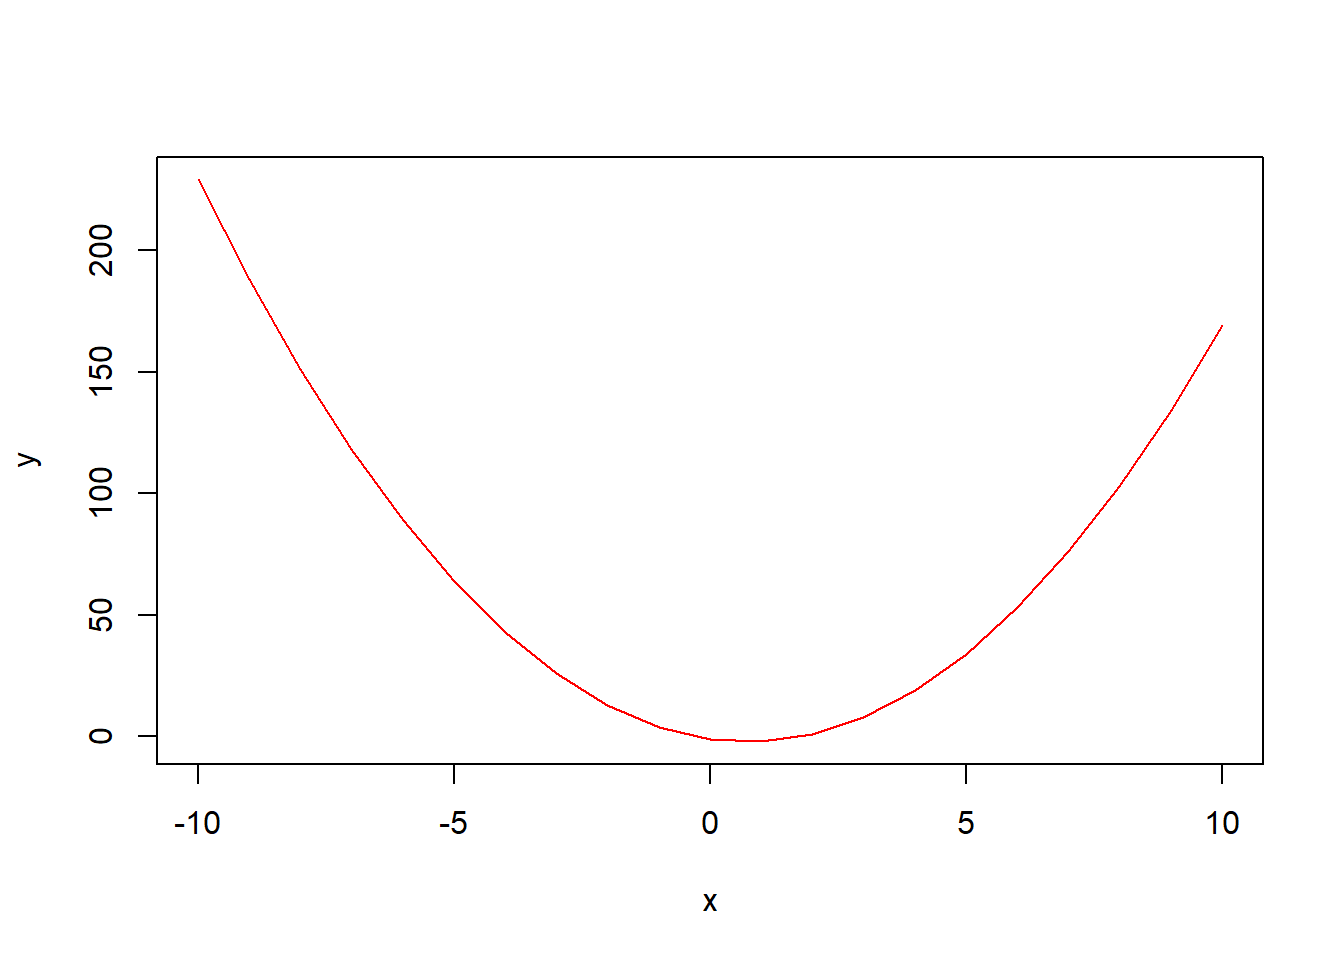
\includegraphics{index_files/figure-latex/unnamed-chunk-16-2.pdf}

\hypertarget{simulations}{%
\chapter{Simulations}\label{simulations}}

R is widely used for simulations due to its extensive set of statistical and mathematical functions, ease of coding, and strong support for random number generation. R's flexibility allows researchers and analysts to implement various simulation models.

In this class we will use the \textbf{sample} function and the \textbf{replicate} function extensively.

\hypertarget{the-sample-function}{%
\section{The sample function}\label{the-sample-function}}

The \texttt{sample()} function in R is used to randomly sample elements of a vector.
The basic syntax is: for a vector \texttt{x}, \texttt{sample(x,size,replace=FALSE,prob=NULL)}

The arguments: \emph{size}, \emph{replace} and \emph{prob} are optional. If they are not included, size is the length of the vector, replace is \texttt{FALSE} and prob is \texttt{NULL}. In this case, we simply get a random permutation of the vector. For example

\begin{Shaded}
\begin{Highlighting}[]
\FunctionTok{sample}\NormalTok{(}\DecValTok{1}\SpecialCharTok{:}\DecValTok{6}\NormalTok{)}
\CommentTok{\#\textgreater{} [1] 1 5 4 2 3 6}
\end{Highlighting}
\end{Shaded}

The sample function can be used to simulate several experiments

\hypertarget{getting-objects-out-of-a-box}{%
\subsection*{Getting objects out of a Box}\label{getting-objects-out-of-a-box}}
\addcontentsline{toc}{subsection}{Getting objects out of a Box}

Suppose that we have a box with 3 red balls, 2 yellow ones and 1 green. We represent the box by the vector

\begin{verbatim}
box <- c("red","red","red","yellow","yellow","green")
\end{verbatim}

\begin{enumerate}
\def\labelenumi{\arabic{enumi}.}
\tightlist
\item
  To randomly select one ball from the box we write \texttt{sample(box,1)}
\item
  To randomly select two balls from the box we write \texttt{sample(box,2)}. Notice that this doesn't include replacement. We either take two balls, or we take one ball and then another one.
\item
  To select two balls with replacement means that we select one ball. We look at it. Put it back in the box and then select a second one at random. To do this we write \texttt{sample(box,2,replace=T)}.
\end{enumerate}

\hypertarget{rolling-dice}{%
\subsection*{Rolling dice}\label{rolling-dice}}
\addcontentsline{toc}{subsection}{Rolling dice}

\begin{enumerate}
\def\labelenumi{\arabic{enumi}.}
\tightlist
\item
  To roll a die we write \texttt{sample(1:6,1)}
\item
  To roll two dice we write \texttt{sample(1:6,2,replace=TRUE)}. Notice that we need to add \texttt{replace=TRUE} because we can get the same number.
\end{enumerate}

\hypertarget{selecting-a-birthday-at-random}{%
\subsection*{Selecting a birthday at random}\label{selecting-a-birthday-at-random}}
\addcontentsline{toc}{subsection}{Selecting a birthday at random}

\begin{enumerate}
\def\labelenumi{\arabic{enumi}.}
\tightlist
\item
  To select a birthday at random we write \texttt{sample(1:365,1)}. We ignore leap years and assume that birthdays are described by numbers from 1 to 365. January 1st is 1. January 2nd is 2, etc.
\item
  To select 10 birthdays at random, we write \texttt{sample(1:365,10,replace=T)}. Notice that we need to add the replace parameter since birthdays can be the same.
\item
  If we want to select 10 \textbf{different} birthdays at random, we write \texttt{sample(1:365,10)}.
\end{enumerate}

\hypertarget{getting-objects-out-of-a-box-using-the-prob-argument}{%
\subsection*{Getting objects out of a Box using the prob Argument}\label{getting-objects-out-of-a-box-using-the-prob-argument}}
\addcontentsline{toc}{subsection}{Getting objects out of a Box using the prob Argument}

The following is an alternative way to select one ball at random from a box that contains 3 red balls, 2 yellow ones and 1 green.

\begin{Shaded}
\begin{Highlighting}[]
\FunctionTok{sample}\NormalTok{(}\FunctionTok{c}\NormalTok{(}\StringTok{"red"}\NormalTok{,}\StringTok{"yellow"}\NormalTok{,}\StringTok{"green"}\NormalTok{),}\DecValTok{1}\NormalTok{,}\AttributeTok{prob =} \FunctionTok{c}\NormalTok{(}\DecValTok{3}\NormalTok{,}\DecValTok{2}\NormalTok{,}\DecValTok{1}\NormalTok{))}
\CommentTok{\#\textgreater{} [1] "yellow"}
\end{Highlighting}
\end{Shaded}

The optional \emph{prob} argument is assigned a vector of weights for obtaining the elements of the vector being sampled. They do not need to sum to one.

\hypertarget{simulating-a-test-with-false-positives-and-false-negatives}{%
\subsection*{Simulating a Test with False Positives and False Negatives}\label{simulating-a-test-with-false-positives-and-false-negatives}}
\addcontentsline{toc}{subsection}{Simulating a Test with False Positives and False Negatives}

Consider a diagnostic test for a specific medical condition. The test identifies individuals with the disease 90\% of the time. However, it also wrongly identifies individuals without the disease as positive 8\% of the time. This test has a 10\% false negative rate and a 8\% false positive rate.

Let's simulate this test in R. We start by agreeing that the input is 0 or 1 (0 means that the person doesn't have the disease and 1 means that the person has the disease) and that the output is also 0 and 1 (0 means the test is negative and 1 means the test is positive).

\begin{Shaded}
\begin{Highlighting}[]
\NormalTok{test }\OtherTok{\textless{}{-}} \ControlFlowTok{function}\NormalTok{(x)\{}
  \ControlFlowTok{if}\NormalTok{ (x}\SpecialCharTok{==}\DecValTok{1}\NormalTok{) \{}
\NormalTok{    value }\OtherTok{=} \FunctionTok{sample}\NormalTok{(}\FunctionTok{c}\NormalTok{(}\DecValTok{0}\NormalTok{,}\DecValTok{1}\NormalTok{),}\DecValTok{1}\NormalTok{,}\AttributeTok{prob =} \FunctionTok{c}\NormalTok{(}\FloatTok{0.1}\NormalTok{,}\FloatTok{0.9}\NormalTok{))}
\NormalTok{  \} }\ControlFlowTok{else}\NormalTok{ \{}
\NormalTok{    value }\OtherTok{=} \FunctionTok{sample}\NormalTok{(}\FunctionTok{c}\NormalTok{(}\DecValTok{0}\NormalTok{,}\DecValTok{1}\NormalTok{),}\DecValTok{1}\NormalTok{,}\AttributeTok{prob =} \FunctionTok{c}\NormalTok{(}\FloatTok{0.92}\NormalTok{,}\FloatTok{0.08}\NormalTok{))}
\NormalTok{  \}}
  \FunctionTok{return}\NormalTok{(value)}
\NormalTok{\}}
\end{Highlighting}
\end{Shaded}

Let's see the results of the test on 40 \textbf{healthy} people. We use the \texttt{rep(\ )} function. Notice that the function \texttt{test} has conditionals. To \protect\hyperlink{vectorize}{vectorize it}, we use the \texttt{sapply} base R function as was \protect\hyperlink{vectorize}{described before}

\begin{Shaded}
\begin{Highlighting}[]
\NormalTok{healthy }\OtherTok{\textless{}{-}} \FunctionTok{rep}\NormalTok{(}\DecValTok{0}\NormalTok{,}\DecValTok{40}\NormalTok{)}
\NormalTok{healthy}
\CommentTok{\#\textgreater{}  [1] 0 0 0 0 0 0 0 0 0 0 0 0 0 0 0 0 0 0 0 0 0 0 0 0 0 0 0 0}
\CommentTok{\#\textgreater{} [29] 0 0 0 0 0 0 0 0 0 0 0 0}
\NormalTok{resultsH }\OtherTok{\textless{}{-}} \FunctionTok{sapply}\NormalTok{(healthy, test)}
\NormalTok{resultsH}
\CommentTok{\#\textgreater{}  [1] 0 0 0 0 0 1 1 0 1 0 0 0 0 0 0 0 0 0 0 0 0 0 0 0 0 0 0 0}
\CommentTok{\#\textgreater{} [29] 0 0 0 0 0 0 0 0 0 0 0 0}
\end{Highlighting}
\end{Shaded}

And now let's see the results on 40 \textbf{sick} people

\begin{Shaded}
\begin{Highlighting}[]
\NormalTok{sick }\OtherTok{\textless{}{-}} \FunctionTok{rep}\NormalTok{(}\DecValTok{1}\NormalTok{,}\DecValTok{30}\NormalTok{)}
\NormalTok{sick}
\CommentTok{\#\textgreater{}  [1] 1 1 1 1 1 1 1 1 1 1 1 1 1 1 1 1 1 1 1 1 1 1 1 1 1 1 1 1}
\CommentTok{\#\textgreater{} [29] 1 1}
\NormalTok{resultsS }\OtherTok{\textless{}{-}} \FunctionTok{sapply}\NormalTok{(sick, test)}
\NormalTok{resultsS}
\CommentTok{\#\textgreater{}  [1] 1 1 0 1 1 1 1 1 1 1 1 1 0 1 1 0 1 1 1 0 1 1 1 1 1 1 1 1}
\CommentTok{\#\textgreater{} [29] 1 1}
\end{Highlighting}
\end{Shaded}

\hypertarget{the-replicate-function}{%
\section{The Replicate Function}\label{the-replicate-function}}

The \texttt{replicate(\ )} function in R is used to replicate the execution of an expression or a function multiple times. The basic syntax is \texttt{replicate(n,expression)}. For example

\begin{enumerate}
\def\labelenumi{\arabic{enumi}.}
\tightlist
\item
  To roll a die 10 times we write \texttt{replicate(10,sample(1:6,1))}. We can also do this using the sample function.
\item
  To select 1 ball from the box 10 times, we write \texttt{replicate(10,sample(box,1))}.
\end{enumerate}

\hypertarget{simulating-experiments}{%
\section{Simulating Experiments}\label{simulating-experiments}}

We combine the sample function, the replicate function and vector functions to simulate more complicated experiments. We illustrate this with these examples:

\begin{example}
Roll a die 20 times and count the number of 6's.
\end{example}

First we roll a die 20 times

\begin{Shaded}
\begin{Highlighting}[]
\NormalTok{values }\OtherTok{\textless{}{-}} \FunctionTok{sample}\NormalTok{(}\DecValTok{1}\SpecialCharTok{:}\DecValTok{6}\NormalTok{,}\DecValTok{20}\NormalTok{,}\AttributeTok{replace =}\NormalTok{ T)}
\NormalTok{values}
\CommentTok{\#\textgreater{}  [1] 4 2 5 3 1 3 4 3 2 2 5 3 3 6 3 6 4 6 2 1}
\end{Highlighting}
\end{Shaded}

Then we check the values that are equal to 6

\begin{Shaded}
\begin{Highlighting}[]
\NormalTok{values }\SpecialCharTok{==} \DecValTok{6}
\CommentTok{\#\textgreater{}  [1] FALSE FALSE FALSE FALSE FALSE FALSE FALSE FALSE FALSE}
\CommentTok{\#\textgreater{} [10] FALSE FALSE FALSE FALSE  TRUE FALSE  TRUE FALSE  TRUE}
\CommentTok{\#\textgreater{} [19] FALSE FALSE}
\end{Highlighting}
\end{Shaded}

R treats \texttt{FALSE} values as 0's and \texttt{TRUE} values as 1's. If we sum these values we find out the number of 6's

\begin{Shaded}
\begin{Highlighting}[]
\FunctionTok{sum}\NormalTok{(values }\SpecialCharTok{==} \DecValTok{6}\NormalTok{)}
\CommentTok{\#\textgreater{} [1] 3}
\end{Highlighting}
\end{Shaded}

\begin{example}
Run the previous experiment 100 times and find the average.
\end{example}

We use the replicate function to run the experiment 100 times and then we use the \texttt{mean()} function to find the average

\begin{Shaded}
\begin{Highlighting}[]
\NormalTok{exper }\OtherTok{\textless{}{-}}\FunctionTok{replicate}\NormalTok{(}\DecValTok{100}\NormalTok{,}\FunctionTok{sum}\NormalTok{(}\FunctionTok{sample}\NormalTok{(}\DecValTok{1}\SpecialCharTok{:}\DecValTok{6}\NormalTok{,}\DecValTok{20}\NormalTok{,}\AttributeTok{replace=}\NormalTok{T) }\SpecialCharTok{==} \DecValTok{6}\NormalTok{))}
\NormalTok{exper }
\CommentTok{\#\textgreater{}   [1] 3 2 2 4 6 2 0 5 5 1 4 4 5 2 2 1 4 3 2 6 2 2 2 3 0 1 6}
\CommentTok{\#\textgreater{}  [28] 5 3 5 3 1 5 4 4 3 2 2 4 2 0 4 1 2 3 4 7 3 4 1 3 4 2 2}
\CommentTok{\#\textgreater{}  [55] 4 3 4 5 3 4 5 4 5 3 5 2 3 1 2 5 2 3 4 2 5 2 2 3 2 3 2}
\CommentTok{\#\textgreater{}  [82] 3 0 5 2 4 2 3 4 3 5 3 3 2 3 1 5 3 5 4}
\FunctionTok{mean}\NormalTok{(exper)}
\CommentTok{\#\textgreater{} [1] 3.1}
\end{Highlighting}
\end{Shaded}

To simplifying reading the code or to handle more complex situations, we can wrap the expression in curly braces to compute it.

\begin{Shaded}
\begin{Highlighting}[]
\FunctionTok{replicate}\NormalTok{(}\DecValTok{100}\NormalTok{,\{}
\NormalTok{  values }\OtherTok{\textless{}{-}} \FunctionTok{sample}\NormalTok{(}\DecValTok{1}\SpecialCharTok{:}\DecValTok{6}\NormalTok{,}\DecValTok{20}\NormalTok{,}\AttributeTok{replace=}\NormalTok{T)}
  \FunctionTok{sum}\NormalTok{(values }\SpecialCharTok{==} \DecValTok{6}\NormalTok{)}
\NormalTok{\})}
\CommentTok{\#\textgreater{}   [1] 3 4 2 1 4 2 3 0 5 4 2 5 4 3 3 3 3 3 3 2 6 3 3 7 5 2 2}
\CommentTok{\#\textgreater{}  [28] 4 5 4 3 4 3 2 2 3 0 5 5 2 6 2 2 3 3 4 0 5 5 2 2 1 4 4}
\CommentTok{\#\textgreater{}  [55] 6 2 3 6 3 2 2 1 4 3 3 2 1 1 2 2 2 4 1 5 3 2 4 5 1 4 5}
\CommentTok{\#\textgreater{}  [82] 4 5 1 5 3 7 2 8 4 3 4 6 3 2 3 4 6 1 3}
\end{Highlighting}
\end{Shaded}

By default, the function replicates the value of the last line

\begin{Shaded}
\begin{Highlighting}[]
\FunctionTok{replicate}\NormalTok{(}\DecValTok{100}\NormalTok{,\{}
\NormalTok{  values }\OtherTok{\textless{}{-}} \FunctionTok{sample}\NormalTok{(}\DecValTok{1}\SpecialCharTok{:}\DecValTok{6}\NormalTok{,}\DecValTok{20}\NormalTok{,}\AttributeTok{replace=}\NormalTok{T)}
  \FunctionTok{sum}\NormalTok{(values }\SpecialCharTok{==} \DecValTok{6}\NormalTok{)}
  \DecValTok{8}
\NormalTok{\})}
\CommentTok{\#\textgreater{}   [1] 8 8 8 8 8 8 8 8 8 8 8 8 8 8 8 8 8 8 8 8 8 8 8 8 8 8 8}
\CommentTok{\#\textgreater{}  [28] 8 8 8 8 8 8 8 8 8 8 8 8 8 8 8 8 8 8 8 8 8 8 8 8 8 8 8}
\CommentTok{\#\textgreater{}  [55] 8 8 8 8 8 8 8 8 8 8 8 8 8 8 8 8 8 8 8 8 8 8 8 8 8 8 8}
\CommentTok{\#\textgreater{}  [82] 8 8 8 8 8 8 8 8 8 8 8 8 8 8 8 8 8 8 8}
\end{Highlighting}
\end{Shaded}

\hypertarget{project-1}{%
\chapter{Project 1}\label{project-1}}

Use R to simulate the following:

\begin{enumerate}
\def\labelenumi{\arabic{enumi}.}
\tightlist
\item
  Roll a dice 4 times and find the sum
\item
  Select 4 different numbers between 1 and 100. Find the maximum value, the minimum value, and the difference.
\item
  Roll 3 dice 100 times. Find how many times the sum of the dice is at least 10.
\item
  Permute the letters of the word SIMULATE 100 times and find out how many times the first letter is an S and the last letter is an E. That is, we are looking for words of the form S******E.
\item
  Repeat the previous problem but find out how many times the first letter is a vowel.
\item
  A box has 4 red balls and 6 blue balls. Select 5 balls 10000 times and find out how many times we get exactly 3 red balls.
\item
  In a popular carnival game, players roll three dice. If at least one of them is a 6, they win \$1; otherwise, they lose \$1. They argue that this is a fair game. Each die has a 1/6 chance of being a 6, and the probability of having at least one 6 in three dice rolls is 1/6 + 1/6 + 1/6 = 1/2. Simulate the game in R. Play it 1000 times and find out how much money you won or lost.
\end{enumerate}

\hypertarget{introduction-to-data-frame}{%
\chapter{Introduction to Data Frame}\label{introduction-to-data-frame}}

\hypertarget{data-frames}{%
\section{Data Frames}\label{data-frames}}

Data frames in R are two-dimensional data structures, similar to spreadsheets. They are used to store and manipulate datasets. The key points are:

\begin{enumerate}
\def\labelenumi{\arabic{enumi}.}
\item
  \emph{Structure}: A data frame is a collection of vectors of equal length, where each vector represents a column. Recall that all the elements of a vectors have the same type.
\item
  \emph{Columns}: Different columns can have different data types (numeric, character, factor, etc.).
\item
  \emph{Rows}: Each row corresponds to a separate observation or record in the dataset.
\end{enumerate}

\hypertarget{creating-data-frames}{%
\subsection{Creating Data Frames}\label{creating-data-frames}}

Data frames are created using the \texttt{data.frame()} function or by importing data sources.

One option is to define the column vectors and to combine them into a data frame using the \texttt{data.frame()} function as shown in this example:

\begin{Shaded}
\begin{Highlighting}[]
\NormalTok{name }\OtherTok{=} \FunctionTok{c}\NormalTok{(}\StringTok{"John Smith"}\NormalTok{,}\StringTok{"Jane Doe"}\NormalTok{, }\StringTok{"Mary Johnson"}\NormalTok{)}
\NormalTok{a }\OtherTok{\textless{}{-}} \FunctionTok{c}\NormalTok{(}\ConstantTok{NaN}\NormalTok{,}\DecValTok{16}\NormalTok{,}\DecValTok{3}\NormalTok{)}
\NormalTok{b}\OtherTok{\textless{}{-}} \FunctionTok{c}\NormalTok{(}\DecValTok{2}\NormalTok{,}\DecValTok{11}\NormalTok{,}\DecValTok{1}\NormalTok{)}
\NormalTok{df1 }\OtherTok{\textless{}{-}} \FunctionTok{data.frame}\NormalTok{(name,a,b)}
\NormalTok{knitr}\SpecialCharTok{::}\FunctionTok{kable}\NormalTok{(df1)}
\end{Highlighting}
\end{Shaded}

\begin{tabular}{l|r|r}
\hline
name & a & b\\
\hline
John Smith & NaN & 2\\
\hline
Jane Doe & 16 & 11\\
\hline
Mary Johnson & 3 & 1\\
\hline
\end{tabular}

We used the \texttt{knitr::kable()} function to have a nicer display.

Data frames can also be defined inside the data.frame() function directly, naming the columns and the values.

\begin{Shaded}
\begin{Highlighting}[]
\NormalTok{df2 }\OtherTok{\textless{}{-}} \FunctionTok{data.frame}\NormalTok{(}
  \AttributeTok{name =} \FunctionTok{c}\NormalTok{(}\StringTok{"John Smith"}\NormalTok{,}\StringTok{"Jane Doe"}\NormalTok{,}\StringTok{"Mary Johnson"}\NormalTok{,}\StringTok{"John Smith"}\NormalTok{,}\StringTok{"Jane Doe"}\NormalTok{,}\StringTok{"Mary Johnson"}\NormalTok{),}
  \AttributeTok{treatment =}\FunctionTok{c}\NormalTok{(}\StringTok{"a"}\NormalTok{,}\StringTok{"a"}\NormalTok{,}\StringTok{"a"}\NormalTok{,}\StringTok{"b"}\NormalTok{,}\StringTok{"b"}\NormalTok{,}\StringTok{"b"}\NormalTok{),}
  \AttributeTok{results =} \FunctionTok{c}\NormalTok{(}\ConstantTok{NaN}\NormalTok{,}\DecValTok{16}\NormalTok{,}\DecValTok{3}\NormalTok{,}\DecValTok{2}\NormalTok{,}\DecValTok{11}\NormalTok{,}\DecValTok{1}\NormalTok{)}
\NormalTok{)}
\NormalTok{knitr}\SpecialCharTok{::}\FunctionTok{kable}\NormalTok{(df2)}
\end{Highlighting}
\end{Shaded}

\begin{tabular}{l|l|r}
\hline
name & treatment & results\\
\hline
John Smith & a & NaN\\
\hline
Jane Doe & a & 16\\
\hline
Mary Johnson & a & 3\\
\hline
John Smith & b & 2\\
\hline
Jane Doe & b & 11\\
\hline
Mary Johnson & b & 1\\
\hline
\end{tabular}

Notice that the data frames df1 and df2 have the same information. We will later learn that df2 is preferred over df1. We will learn how to convert a data frame like df1 into a data frame like df2. df2 has a ``tidy'' format that fits specially well with many libraries of R.

\hypertarget{importing-data-sets-from-r-head-and-tail}{%
\subsection*{Importing data sets from R, head(), and tail()}\label{importing-data-sets-from-r-head-and-tail}}
\addcontentsline{toc}{subsection}{Importing data sets from R, head(), and tail()}

R has several data sets that can be imported using the \texttt{data()} function. If you write data() inside an R block and run it, you will see a list of all data sets.

For illustration, we will import the iris data set that has 150 rows. We will use the \texttt{head()} function to see only the first 6 rows. The \texttt{tail()} function is similar, but it shows the last 6 rows by default.

\begin{Shaded}
\begin{Highlighting}[]
\FunctionTok{data}\NormalTok{(iris)}
\FunctionTok{head}\NormalTok{(iris) }
\CommentTok{\#\textgreater{}   Sepal.Length Sepal.Width Petal.Length Petal.Width Species}
\CommentTok{\#\textgreater{} 1          5.1         3.5          1.4         0.2  setosa}
\CommentTok{\#\textgreater{} 2          4.9         3.0          1.4         0.2  setosa}
\CommentTok{\#\textgreater{} 3          4.7         3.2          1.3         0.2  setosa}
\CommentTok{\#\textgreater{} 4          4.6         3.1          1.5         0.2  setosa}
\CommentTok{\#\textgreater{} 5          5.0         3.6          1.4         0.2  setosa}
\CommentTok{\#\textgreater{} 6          5.4         3.9          1.7         0.4  setosa}
\end{Highlighting}
\end{Shaded}

\hypertarget{extracting-columns-from-a-data-frame}{%
\subsection*{Extracting columns from a data frame}\label{extracting-columns-from-a-data-frame}}
\addcontentsline{toc}{subsection}{Extracting columns from a data frame}

The syntax to extract columns is data\_frame\$column\_name. Recall that the columns of a data frame are vectors.

\begin{Shaded}
\begin{Highlighting}[]
\NormalTok{iris}\SpecialCharTok{$}\NormalTok{Sepal.Length}
\CommentTok{\#\textgreater{}   [1] 5.1 4.9 4.7 4.6 5.0 5.4 4.6 5.0 4.4 4.9 5.4 4.8 4.8}
\CommentTok{\#\textgreater{}  [14] 4.3 5.8 5.7 5.4 5.1 5.7 5.1 5.4 5.1 4.6 5.1 4.8 5.0}
\CommentTok{\#\textgreater{}  [27] 5.0 5.2 5.2 4.7 4.8 5.4 5.2 5.5 4.9 5.0 5.5 4.9 4.4}
\CommentTok{\#\textgreater{}  [40] 5.1 5.0 4.5 4.4 5.0 5.1 4.8 5.1 4.6 5.3 5.0 7.0 6.4}
\CommentTok{\#\textgreater{}  [53] 6.9 5.5 6.5 5.7 6.3 4.9 6.6 5.2 5.0 5.9 6.0 6.1 5.6}
\CommentTok{\#\textgreater{}  [66] 6.7 5.6 5.8 6.2 5.6 5.9 6.1 6.3 6.1 6.4 6.6 6.8 6.7}
\CommentTok{\#\textgreater{}  [79] 6.0 5.7 5.5 5.5 5.8 6.0 5.4 6.0 6.7 6.3 5.6 5.5 5.5}
\CommentTok{\#\textgreater{}  [92] 6.1 5.8 5.0 5.6 5.7 5.7 6.2 5.1 5.7 6.3 5.8 7.1 6.3}
\CommentTok{\#\textgreater{} [105] 6.5 7.6 4.9 7.3 6.7 7.2 6.5 6.4 6.8 5.7 5.8 6.4 6.5}
\CommentTok{\#\textgreater{} [118] 7.7 7.7 6.0 6.9 5.6 7.7 6.3 6.7 7.2 6.2 6.1 6.4 7.2}
\CommentTok{\#\textgreater{} [131] 7.4 7.9 6.4 6.3 6.1 7.7 6.3 6.4 6.0 6.9 6.7 6.9 5.8}
\CommentTok{\#\textgreater{} [144] 6.8 6.7 6.7 6.3 6.5 6.2 5.9}
\end{Highlighting}
\end{Shaded}

\hypertarget{some-data-frame-functions}{%
\subsection*{Some Data Frame Functions}\label{some-data-frame-functions}}
\addcontentsline{toc}{subsection}{Some Data Frame Functions}

The following is a list of some of the most useful data frame functions. In the next section we will import the library dplyr. This library handles functions 9-14 in a nicer way.

\begin{enumerate}
\def\labelenumi{\arabic{enumi}.}
\tightlist
\item
  head(): Displays the first few rows of a data frame.
\item
  tail(): Displays the last few rows of a data frame.
\item
  str(): Shows the structure of a data frame.
\item
  summary(): Provides summary statistics for each column.
\item
  nrow(): Returns the number of rows in a data frame.
\item
  ncol(): Returns the number of columns in a data frame.
\item
  colnames(): Returns or sets the column names.
\item
  rownames(): Returns or sets the row names.
\item
  subset(): Subsets a data frame based on conditions.
  subset(df, condition)
\item
  select(): Chooses specific columns.
  select(df, column1, column2)
\item
  filter(): Filters rows based on conditions.
  filter(df, condition)
\item
  mutate(): Adds new variables or modifies existing ones.
  mutate(df, new\_column = expression)
\item
  arrange(): Sorts rows based on one or more columns.
  arrange(df, column1, column2)
\item
  merge(): Combines two data frames by common columns.
  merge(df1, df2, by = ``common\_column'')
\end{enumerate}

We will illustrate some of these functions with the data frame iris.

\begin{Shaded}
\begin{Highlighting}[]
\FunctionTok{str}\NormalTok{(iris) }\CommentTok{\#str shows the structure of the data set.}
\CommentTok{\#\textgreater{} \textquotesingle{}data.frame\textquotesingle{}:    150 obs. of  5 variables:}
\CommentTok{\#\textgreater{}  $ Sepal.Length: num  5.1 4.9 4.7 4.6 5 5.4 4.6 5 4.4 4.9 ...}
\CommentTok{\#\textgreater{}  $ Sepal.Width : num  3.5 3 3.2 3.1 3.6 3.9 3.4 3.4 2.9 3.1 ...}
\CommentTok{\#\textgreater{}  $ Petal.Length: num  1.4 1.4 1.3 1.5 1.4 1.7 1.4 1.5 1.4 1.5 ...}
\CommentTok{\#\textgreater{}  $ Petal.Width : num  0.2 0.2 0.2 0.2 0.2 0.4 0.3 0.2 0.2 0.1 ...}
\CommentTok{\#\textgreater{}  $ Species     : Factor w/ 3 levels "setosa","versicolor",..: 1 1 1 1 1 1 1 1 1 1 ...}
\end{Highlighting}
\end{Shaded}

\begin{Shaded}
\begin{Highlighting}[]
\FunctionTok{summary}\NormalTok{(iris) }\CommentTok{\# summary provides summary statistical for each column.}
\CommentTok{\#\textgreater{}   Sepal.Length    Sepal.Width     Petal.Length  }
\CommentTok{\#\textgreater{}  Min.   :4.300   Min.   :2.000   Min.   :1.000  }
\CommentTok{\#\textgreater{}  1st Qu.:5.100   1st Qu.:2.800   1st Qu.:1.600  }
\CommentTok{\#\textgreater{}  Median :5.800   Median :3.000   Median :4.350  }
\CommentTok{\#\textgreater{}  Mean   :5.843   Mean   :3.057   Mean   :3.758  }
\CommentTok{\#\textgreater{}  3rd Qu.:6.400   3rd Qu.:3.300   3rd Qu.:5.100  }
\CommentTok{\#\textgreater{}  Max.   :7.900   Max.   :4.400   Max.   :6.900  }
\CommentTok{\#\textgreater{}   Petal.Width          Species  }
\CommentTok{\#\textgreater{}  Min.   :0.100   setosa    :50  }
\CommentTok{\#\textgreater{}  1st Qu.:0.300   versicolor:50  }
\CommentTok{\#\textgreater{}  Median :1.300   virginica :50  }
\CommentTok{\#\textgreater{}  Mean   :1.199                  }
\CommentTok{\#\textgreater{}  3rd Qu.:1.800                  }
\CommentTok{\#\textgreater{}  Max.   :2.500}
\end{Highlighting}
\end{Shaded}

\begin{Shaded}
\begin{Highlighting}[]
\FunctionTok{nrow}\NormalTok{(iris) }\CommentTok{\# nrwon finds the number of rows}
\CommentTok{\#\textgreater{} [1] 150}
\end{Highlighting}
\end{Shaded}

\begin{Shaded}
\begin{Highlighting}[]
\FunctionTok{colnames}\NormalTok{(iris) }\CommentTok{\# colnames finds the names of the columns}
\CommentTok{\#\textgreater{} [1] "Sepal.Length" "Sepal.Width"  "Petal.Length"}
\CommentTok{\#\textgreater{} [4] "Petal.Width"  "Species"}
\end{Highlighting}
\end{Shaded}

\hypertarget{dplyr-and-conditional-probability}{%
\chapter{DPLYR and Conditional Probability}\label{dplyr-and-conditional-probability}}

dplyr is a popular R library used to manipulate data consistently and efficiently. It uses a set of functions, that they call ``verbs''. These functions are used to solve the most common data manipulation problems. The main verbs are:

\begin{itemize}
\tightlist
\item
  \emph{mutate} to create new columns. The syntax is
\end{itemize}

\begin{verbatim}
mutate(data_frame, new_column_name = expression)
\end{verbatim}

\begin{itemize}
\tightlist
\item
  \emph{filter} to select rows. The syntax is
\end{itemize}

\begin{verbatim}
filter(data_frame,condition)
\end{verbatim}

\begin{itemize}
\tightlist
\item
  \emph{select} to select columns. The syntax is
\end{itemize}

\begin{verbatim}
select(data_frame, column1,column2,...,columnk)
\end{verbatim}

\begin{itemize}
\tightlist
\item
  \emph{arrange} reorders the rows. The syntax is
\end{itemize}

\begin{verbatim}
arange(data_frame,column1,columns2,...)
\end{verbatim}

These functions are combined with group\_by() and summarise() to easily perform group-wise operations and compute summary statistics within those groups.

To use a library we type library(name\_of\_library). If the library is not intalled, we install it through Packages in RStudio.

\hypertarget{conditional-probability-dice}{%
\section{Conditional Probability - dice}\label{conditional-probability-dice}}

\begin{example}
You roll two dice. Estimate the conditional probability that the first die is 6 if the sum is 10
\end{example}

Step 1: Select a large number of simulations and generate the dice data.

\begin{Shaded}
\begin{Highlighting}[]
\NormalTok{n }\OtherTok{\textless{}{-}} \DecValTok{10000}
\NormalTok{die1 }\OtherTok{\textless{}{-}} \FunctionTok{sample}\NormalTok{(}\DecValTok{1}\SpecialCharTok{:}\DecValTok{6}\NormalTok{,n,}\AttributeTok{replace =}\NormalTok{ T)}
\NormalTok{die2 }\OtherTok{\textless{}{-}} \FunctionTok{sample}\NormalTok{(}\DecValTok{1}\SpecialCharTok{:}\DecValTok{6}\NormalTok{,n,}\AttributeTok{replace =}\NormalTok{ T)}
\end{Highlighting}
\end{Shaded}

Step 2: Make the data into a dataframe.

\begin{Shaded}
\begin{Highlighting}[]
\NormalTok{df }\OtherTok{\textless{}{-}} \FunctionTok{data.frame}\NormalTok{(die1,die2)}
\FunctionTok{head}\NormalTok{(df)}
\CommentTok{\#\textgreater{}   die1 die2}
\CommentTok{\#\textgreater{} 1    6    6}
\CommentTok{\#\textgreater{} 2    2    5}
\CommentTok{\#\textgreater{} 3    4    3}
\CommentTok{\#\textgreater{} 4    1    1}
\CommentTok{\#\textgreater{} 5    5    6}
\CommentTok{\#\textgreater{} 6    2    2}
\end{Highlighting}
\end{Shaded}

Step 3: Use mutate to create a new column that includes the sum.

\begin{Shaded}
\begin{Highlighting}[]
\NormalTok{dfm }\OtherTok{\textless{}{-}} \FunctionTok{mutate}\NormalTok{(df,}\AttributeTok{sum =}\NormalTok{ die1}\SpecialCharTok{+}\NormalTok{die2)}
\FunctionTok{head}\NormalTok{(dfm)}
\CommentTok{\#\textgreater{}   die1 die2 sum}
\CommentTok{\#\textgreater{} 1    6    6  12}
\CommentTok{\#\textgreater{} 2    2    5   7}
\CommentTok{\#\textgreater{} 3    4    3   7}
\CommentTok{\#\textgreater{} 4    1    1   2}
\CommentTok{\#\textgreater{} 5    5    6  11}
\CommentTok{\#\textgreater{} 6    2    2   4}
\end{Highlighting}
\end{Shaded}

Step 4: Select the rows that add up to ten. This is the key point of conditional probability.

\begin{Shaded}
\begin{Highlighting}[]
\NormalTok{dff }\OtherTok{\textless{}{-}} \FunctionTok{filter}\NormalTok{(dfm,sum }\SpecialCharTok{==} \DecValTok{10}\NormalTok{)}
\FunctionTok{head}\NormalTok{(dff)}
\CommentTok{\#\textgreater{}   die1 die2 sum}
\CommentTok{\#\textgreater{} 1    5    5  10}
\CommentTok{\#\textgreater{} 2    4    6  10}
\CommentTok{\#\textgreater{} 3    6    4  10}
\CommentTok{\#\textgreater{} 4    4    6  10}
\CommentTok{\#\textgreater{} 5    6    4  10}
\CommentTok{\#\textgreater{} 6    4    6  10}
\end{Highlighting}
\end{Shaded}

Step 5: Extract the column that has the first die, and find the proportion of sixes.

\begin{Shaded}
\begin{Highlighting}[]
\FunctionTok{mean}\NormalTok{(dff}\SpecialCharTok{$}\NormalTok{die1 }\SpecialCharTok{==} \DecValTok{6}\NormalTok{)}
\CommentTok{\#\textgreater{} [1] 0.3277108}
\end{Highlighting}
\end{Shaded}

\hypertarget{the-pipe-operator-in-dplyr}{%
\section{The Pipe Operator (\%\textgreater\%) in DPLYR}\label{the-pipe-operator-in-dplyr}}

Saving new dataframes every time we perform new operations is tedious and it can be confusing. In dplyr, the pipe operator (\%\textgreater\%) passes the result of one operation as the first argument to another operation. This improves code readability by creating a concise syntax that chains multiple operations together.

For example, these four lines reproduce the previous operations and it adds a new column named \textbf{\emph{experiment}} that checks if die1 is equal to 6.

\begin{Shaded}
\begin{Highlighting}[]
\NormalTok{df }\SpecialCharTok{\%\textgreater{}\%} 
  \FunctionTok{mutate}\NormalTok{(}\AttributeTok{sum =}\NormalTok{ die1}\SpecialCharTok{+}\NormalTok{die2) }\SpecialCharTok{\%\textgreater{}\%}
  \FunctionTok{filter}\NormalTok{(sum }\SpecialCharTok{==} \DecValTok{10}\NormalTok{) }\SpecialCharTok{\%\textgreater{}\%}
  \FunctionTok{mutate}\NormalTok{(}\AttributeTok{experiment =}\NormalTok{ die1 }\SpecialCharTok{==} \DecValTok{6}\NormalTok{) }\SpecialCharTok{\%\textgreater{}\%}
  \FunctionTok{head}\NormalTok{()}
\CommentTok{\#\textgreater{}   die1 die2 sum experiment}
\CommentTok{\#\textgreater{} 1    5    5  10      FALSE}
\CommentTok{\#\textgreater{} 2    4    6  10      FALSE}
\CommentTok{\#\textgreater{} 3    6    4  10       TRUE}
\CommentTok{\#\textgreater{} 4    4    6  10      FALSE}
\CommentTok{\#\textgreater{} 5    6    4  10       TRUE}
\CommentTok{\#\textgreater{} 6    4    6  10      FALSE}
\end{Highlighting}
\end{Shaded}

\hypertarget{conditional-probability-test}{%
\section{Conditional Probability - test for disease}\label{conditional-probability-test}}

\begin{example}
A new test was developed for a disease that only 1\% of the population has. The test identifies individuals with the disease 90\% of the time. However, it also wrongly identifies individuals without the disease as positive 5\% of the time. Estimate the probability that a person who tests positive for the disease actually has the disease.
\end{example}

Notice that this test has a 10\% false negative rate and a 5\% false positive rate.

We first choose a large number of simulations and then proceed to randomly assign individuals. Each person is assigned a value of 1 with a probability of 1\%, indicating the presence of the disease, or 0 with a probability of 99\%, signifying the absence of the disease.

\begin{Shaded}
\begin{Highlighting}[]
\NormalTok{n }\OtherTok{\textless{}{-}} \DecValTok{100000}
\NormalTok{people }\OtherTok{\textless{}{-}} \FunctionTok{sample}\NormalTok{(}\FunctionTok{c}\NormalTok{(}\DecValTok{0}\NormalTok{,}\DecValTok{1}\NormalTok{),n,}\AttributeTok{replace =}\NormalTok{ T,}\AttributeTok{prob =} \FunctionTok{c}\NormalTok{(}\FloatTok{0.99}\NormalTok{,}\FloatTok{0.01}\NormalTok{)) }
\end{Highlighting}
\end{Shaded}

Then we write the function that simulates the test for the disease.

\begin{Shaded}
\begin{Highlighting}[]
\NormalTok{test }\OtherTok{\textless{}{-}} \ControlFlowTok{function}\NormalTok{(x)\{}
  \ControlFlowTok{if}\NormalTok{ (x}\SpecialCharTok{==}\DecValTok{1}\NormalTok{) \{}
\NormalTok{    value }\OtherTok{=} \FunctionTok{sample}\NormalTok{(}\FunctionTok{c}\NormalTok{(}\DecValTok{0}\NormalTok{,}\DecValTok{1}\NormalTok{),}\DecValTok{1}\NormalTok{,}\AttributeTok{prob =} \FunctionTok{c}\NormalTok{(}\FloatTok{0.1}\NormalTok{,}\FloatTok{0.9}\NormalTok{))}
\NormalTok{  \} }\ControlFlowTok{else}\NormalTok{ \{}
\NormalTok{    value }\OtherTok{=} \FunctionTok{sample}\NormalTok{(}\FunctionTok{c}\NormalTok{(}\DecValTok{0}\NormalTok{,}\DecValTok{1}\NormalTok{),}\DecValTok{1}\NormalTok{,}\AttributeTok{prob =} \FunctionTok{c}\NormalTok{(}\FloatTok{0.95}\NormalTok{,}\FloatTok{0.05}\NormalTok{))}
\NormalTok{  \}}
  \FunctionTok{return}\NormalTok{(value)}
\NormalTok{\}}
\end{Highlighting}
\end{Shaded}

Now we apply the test to each person. Since the function has conditionals, we use the sapply() function.

\begin{Shaded}
\begin{Highlighting}[]
\NormalTok{results }\OtherTok{\textless{}{-}} \FunctionTok{sapply}\NormalTok{(people, test)}
\end{Highlighting}
\end{Shaded}

\begin{Shaded}
\begin{Highlighting}[]
\NormalTok{df }\OtherTok{\textless{}{-}} \FunctionTok{data.frame}\NormalTok{(people,results)}
\FunctionTok{head}\NormalTok{(df)}
\CommentTok{\#\textgreater{}   people results}
\CommentTok{\#\textgreater{} 1      0       0}
\CommentTok{\#\textgreater{} 2      0       0}
\CommentTok{\#\textgreater{} 3      0       0}
\CommentTok{\#\textgreater{} 4      0       0}
\CommentTok{\#\textgreater{} 5      0       0}
\CommentTok{\#\textgreater{} 6      0       0}
\end{Highlighting}
\end{Shaded}

Now we select the people who tested positive, and we use the base R function \textbf{\emph{table}} to find out how many of them have the disease and how many don't.

The function \textbf{\emph{table}} counts the occurrences of each unique value in a given vector.

\begin{Shaded}
\begin{Highlighting}[]
\NormalTok{positive }\OtherTok{\textless{}{-}} \FunctionTok{filter}\NormalTok{(df,results}\SpecialCharTok{==}\DecValTok{1}\NormalTok{)}
\FunctionTok{head}\NormalTok{(positive)}
\CommentTok{\#\textgreater{}   people results}
\CommentTok{\#\textgreater{} 1      0       1}
\CommentTok{\#\textgreater{} 2      0       1}
\CommentTok{\#\textgreater{} 3      0       1}
\CommentTok{\#\textgreater{} 4      0       1}
\CommentTok{\#\textgreater{} 5      0       1}
\CommentTok{\#\textgreater{} 6      1       1}
\end{Highlighting}
\end{Shaded}

\begin{Shaded}
\begin{Highlighting}[]
\FunctionTok{table}\NormalTok{(positive}\SpecialCharTok{$}\NormalTok{people)}
\CommentTok{\#\textgreater{} }
\CommentTok{\#\textgreater{}    0    1 }
\CommentTok{\#\textgreater{} 5073  867}
\end{Highlighting}
\end{Shaded}

The output of the table function can be plot directly as a pie plot or as a bar plot.

\begin{Shaded}
\begin{Highlighting}[]
\FunctionTok{pie}\NormalTok{(}\FunctionTok{table}\NormalTok{(positive}\SpecialCharTok{$}\NormalTok{people))}
\end{Highlighting}
\end{Shaded}

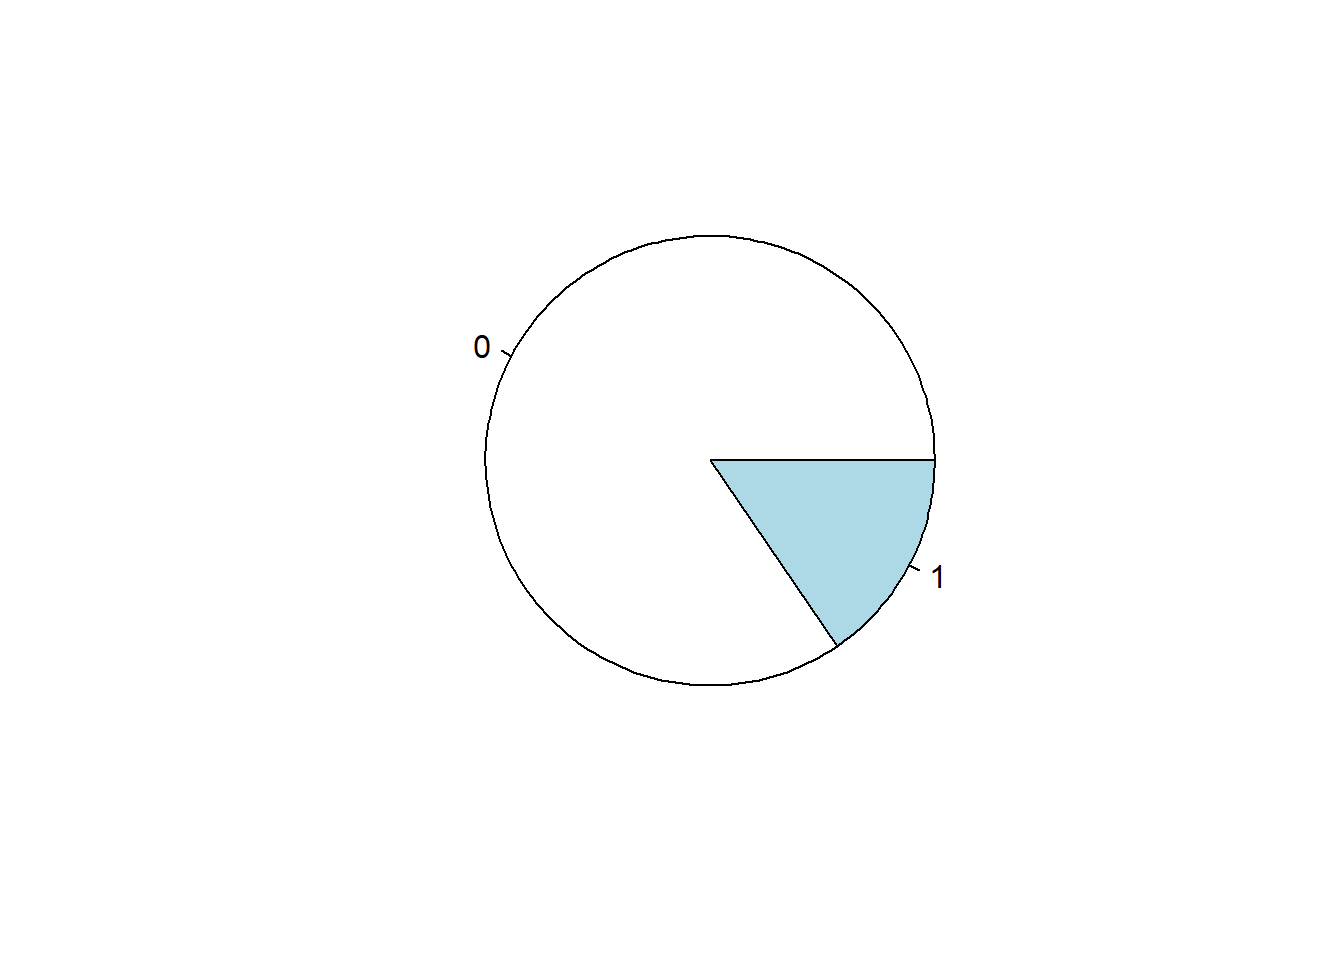
\includegraphics{dplyr_files/figure-latex/unnamed-chunk-14-1.pdf}

\begin{Shaded}
\begin{Highlighting}[]
\FunctionTok{barplot}\NormalTok{(}\FunctionTok{table}\NormalTok{(positive}\SpecialCharTok{$}\NormalTok{people))}
\end{Highlighting}
\end{Shaded}

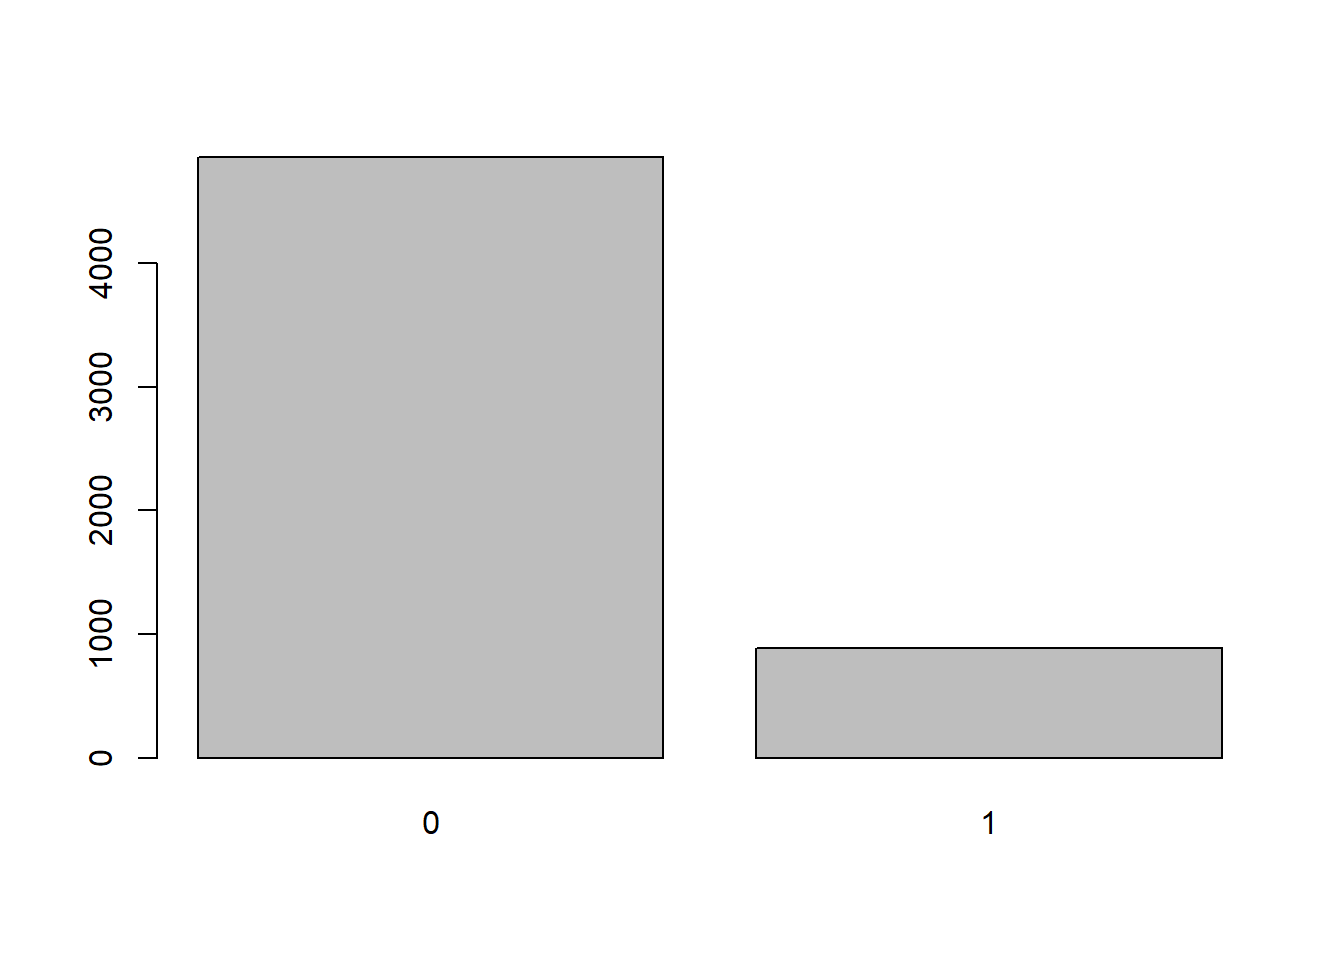
\includegraphics{dplyr_files/figure-latex/unnamed-chunk-14-2.pdf}

We can easily add titles and make the graphs more informative

\begin{Shaded}
\begin{Highlighting}[]
\FunctionTok{pie}\NormalTok{(}\FunctionTok{table}\NormalTok{(positive}\SpecialCharTok{$}\NormalTok{people),}\AttributeTok{main=}\StringTok{"People who tested positive"}\NormalTok{, }\AttributeTok{labels=}\FunctionTok{c}\NormalTok{(}\StringTok{"do not have the disease"}\NormalTok{,}\StringTok{"have the disease"}\NormalTok{), }\AttributeTok{col=}\FunctionTok{c}\NormalTok{(}\StringTok{"\#4CAF50"}\NormalTok{,}\StringTok{"\#FF5252"}\NormalTok{))}
\end{Highlighting}
\end{Shaded}

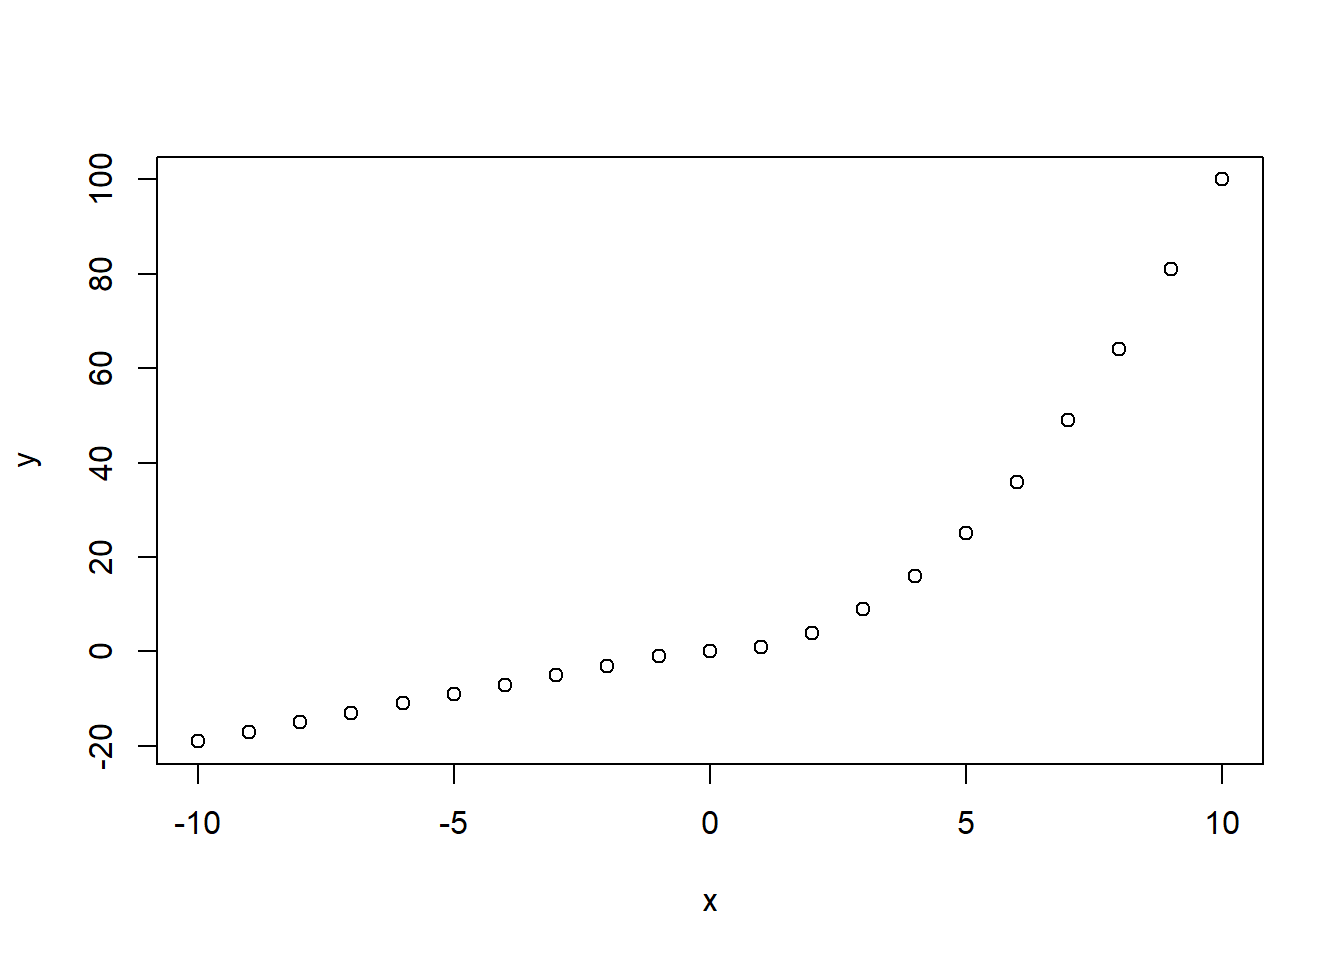
\includegraphics{dplyr_files/figure-latex/unnamed-chunk-15-1.pdf}

\begin{Shaded}
\begin{Highlighting}[]
\FunctionTok{barplot}\NormalTok{(}\FunctionTok{table}\NormalTok{(positive}\SpecialCharTok{$}\NormalTok{people),}\AttributeTok{main=}\StringTok{"People who tested positive"}\NormalTok{, }\AttributeTok{names.arg =} \FunctionTok{c}\NormalTok{(}\StringTok{"do not have the disease"}\NormalTok{,}\StringTok{"have the disease"}\NormalTok{), }\AttributeTok{col=}\FunctionTok{c}\NormalTok{(}\StringTok{"\#4CAF50"}\NormalTok{,}\StringTok{"\#FF5252"}\NormalTok{))}
\end{Highlighting}
\end{Shaded}

\includegraphics{dplyr_files/figure-latex/unnamed-chunk-16-1.pdf}

\hypertarget{row-wise-operations}{%
\chapter{Row Wise Operations}\label{row-wise-operations}}

In R and in dplyr it is easier to perform column operations than row operations. We will illustrate this with the following data frame:

\begin{Shaded}
\begin{Highlighting}[]
\NormalTok{df}
\CommentTok{\#\textgreater{}   x y  z}
\CommentTok{\#\textgreater{} 1 5 1  9}
\CommentTok{\#\textgreater{} 2 6 2 10}
\CommentTok{\#\textgreater{} 3 7 3 11}
\CommentTok{\#\textgreater{} 4 8 4 12}
\end{Highlighting}
\end{Shaded}

If we add the columns using the variables we get the right result.

\begin{Shaded}
\begin{Highlighting}[]
\FunctionTok{mutate}\NormalTok{(df,}\AttributeTok{sum =}\NormalTok{ x}\SpecialCharTok{+}\NormalTok{y}\SpecialCharTok{+}\NormalTok{z)}
\CommentTok{\#\textgreater{}   x y  z sum}
\CommentTok{\#\textgreater{} 1 5 1  9  15}
\CommentTok{\#\textgreater{} 2 6 2 10  18}
\CommentTok{\#\textgreater{} 3 7 3 11  21}
\CommentTok{\#\textgreater{} 4 8 4 12  24}
\end{Highlighting}
\end{Shaded}

On the other hand, if we use vectorized operators (i.e., we convert `\texttt{x,y,z} into a vector and add it), we get the wrong answer. R (or dplyr) computes the sum accross all the rows:

\begin{Shaded}
\begin{Highlighting}[]
\FunctionTok{mutate}\NormalTok{(df, }\AttributeTok{sum =} \FunctionTok{sum}\NormalTok{(}\FunctionTok{c}\NormalTok{(x,y,z)))}
\CommentTok{\#\textgreater{}   x y  z sum}
\CommentTok{\#\textgreater{} 1 5 1  9  78}
\CommentTok{\#\textgreater{} 2 6 2 10  78}
\CommentTok{\#\textgreater{} 3 7 3 11  78}
\CommentTok{\#\textgreater{} 4 8 4 12  78}
\end{Highlighting}
\end{Shaded}

Something similar happens if we use functions.

The following block has four functions. We use the first two to compute the sum of the columns and the last two to select an element from each row. The first function computes the sum adding the variables. The second one vectorizes the variables and adds them. The third function vectorizes the variables and selects one at random, and the last one avoids vectorizing the variables with if then statements.

\begin{Shaded}
\begin{Highlighting}[]
\NormalTok{suma1 }\OtherTok{\textless{}{-}} \ControlFlowTok{function}\NormalTok{(a,b,c)\{}
  \FunctionTok{return}\NormalTok{(a}\SpecialCharTok{+}\NormalTok{b}\SpecialCharTok{+}\NormalTok{c)}
\NormalTok{\}}

\NormalTok{suma2 }\OtherTok{\textless{}{-}} \ControlFlowTok{function}\NormalTok{(vec)\{}
  \FunctionTok{return}\NormalTok{(}\FunctionTok{sum}\NormalTok{(vec))}
\NormalTok{\}}

\NormalTok{choose\_one1 }\OtherTok{\textless{}{-}} \ControlFlowTok{function}\NormalTok{(a,b,c)\{}
  \FunctionTok{return}\NormalTok{(}\FunctionTok{sample}\NormalTok{(}\FunctionTok{c}\NormalTok{(a,b,c),}\DecValTok{1}\NormalTok{))}
\NormalTok{\}}

\NormalTok{choose\_one2 }\OtherTok{\textless{}{-}} \ControlFlowTok{function}\NormalTok{(a,b,c)\{}
\NormalTok{  n }\OtherTok{\textless{}{-}} \FunctionTok{sample}\NormalTok{(}\DecValTok{1}\SpecialCharTok{:}\DecValTok{3}\NormalTok{,}\DecValTok{1}\NormalTok{)}
  \ControlFlowTok{if}\NormalTok{ (n}\SpecialCharTok{==}\DecValTok{1}\NormalTok{)\{}
    \FunctionTok{return}\NormalTok{(a)}
\NormalTok{  \} }\ControlFlowTok{else} \ControlFlowTok{if}\NormalTok{ (n}\SpecialCharTok{==}\DecValTok{2}\NormalTok{)\{}
    \FunctionTok{return}\NormalTok{(b)}
\NormalTok{  \} }\ControlFlowTok{else}\NormalTok{ \{}
    \FunctionTok{return}\NormalTok{(c)}
\NormalTok{  \}}
\NormalTok{\}}
\end{Highlighting}
\end{Shaded}

Then we add a column for each function

\begin{Shaded}
\begin{Highlighting}[]
\FunctionTok{mutate}\NormalTok{(df,}\AttributeTok{sum1 =} \FunctionTok{suma1}\NormalTok{(x,y,z), }\AttributeTok{sum2 =} \FunctionTok{suma2}\NormalTok{(}\FunctionTok{c}\NormalTok{(x,y,z)), }\AttributeTok{choose\_one1 =} \FunctionTok{choose\_one1}\NormalTok{(x,y,z), }\AttributeTok{choose\_one2 =} \FunctionTok{choose\_one2}\NormalTok{(x,y,z))}
\CommentTok{\#\textgreater{}   x y  z sum1 sum2 choose\_one1 choose\_one2}
\CommentTok{\#\textgreater{} 1 5 1  9   15   78           8           1}
\CommentTok{\#\textgreater{} 2 6 2 10   18   78           8           2}
\CommentTok{\#\textgreater{} 3 7 3 11   21   78           8           3}
\CommentTok{\#\textgreater{} 4 8 4 12   24   78           8           4}
\end{Highlighting}
\end{Shaded}

As you see, the first sum works well but he second one doesn't. The other functions don't work well either. \textbf{\emph{choose\_one1}} selected one element from all the rows. \textbf{\emph{choose\_one2}} selected different elements, but all were chosen from the same column.

\hypertarget{rowwise}{%
\section{rowwise()}\label{rowwise}}

To perform row operations properly, we ``group'' the data across each row, using the function \texttt{rowwise()}. We illustrate it's use with the previous data frame and using the pipe operator. We start from the data frame, then we group the data frame by rows, and finally we add the four columns using the previous functions.

\begin{Shaded}
\begin{Highlighting}[]
\NormalTok{df }\SpecialCharTok{\%\textgreater{}\%}
  \FunctionTok{rowwise}\NormalTok{() }\SpecialCharTok{\%\textgreater{}\%}
  \FunctionTok{mutate}\NormalTok{(}\AttributeTok{sum1 =} \FunctionTok{suma1}\NormalTok{(x,y,z),}\AttributeTok{sum2=}\FunctionTok{suma2}\NormalTok{(}\FunctionTok{c}\NormalTok{(x,y,z)),}\AttributeTok{choose\_one1 =} \FunctionTok{choose\_one1}\NormalTok{(x,y,z), }\AttributeTok{choose\_one2 =} \FunctionTok{choose\_one2}\NormalTok{(x,y,z))}
\CommentTok{\#\textgreater{} \# A tibble: 4 x 7}
\CommentTok{\#\textgreater{} \# Rowwise: }
\CommentTok{\#\textgreater{}       x     y     z  sum1  sum2 choose\_one1 choose\_one2}
\CommentTok{\#\textgreater{}   \textless{}dbl\textgreater{} \textless{}dbl\textgreater{} \textless{}dbl\textgreater{} \textless{}dbl\textgreater{} \textless{}dbl\textgreater{}       \textless{}dbl\textgreater{}       \textless{}dbl\textgreater{}}
\CommentTok{\#\textgreater{} 1     5     1     9    15    15           9           9}
\CommentTok{\#\textgreater{} 2     6     2    10    18    18           6          10}
\CommentTok{\#\textgreater{} 3     7     3    11    21    21           3           3}
\CommentTok{\#\textgreater{} 4     8     4    12    24    24           4           4}
\end{Highlighting}
\end{Shaded}

Notice that in this case, all the operations worked well. The last two columns are different because they were selected randomly. Nevertheless, each of them selects one element from each row.

\hypertarget{ungroup}{%
\section{ungroup()}\label{ungroup}}

The \texttt{rowwise()} operator does not change the data, but it groups it. If we look carefully at the output, we see that the table says ``\# Rowwise'' to let us know that the data is grouped by rows. To remove the grouping, we add the \texttt{ungroup()} operator.

\begin{Shaded}
\begin{Highlighting}[]
\NormalTok{df }\SpecialCharTok{\%\textgreater{}\%}
  \FunctionTok{rowwise}\NormalTok{() }\SpecialCharTok{\%\textgreater{}\%}
  \FunctionTok{mutate}\NormalTok{(}\AttributeTok{sum1 =} \FunctionTok{suma1}\NormalTok{(x,y,z),}\AttributeTok{sum2=}\FunctionTok{suma2}\NormalTok{(}\FunctionTok{c}\NormalTok{(x,y,z)),}\AttributeTok{choose\_one1 =} \FunctionTok{choose\_one1}\NormalTok{(x,y,z), }\AttributeTok{choose\_one2 =} \FunctionTok{choose\_one2}\NormalTok{(x,y,z)) }\SpecialCharTok{\%\textgreater{}\%}
  \FunctionTok{ungroup}\NormalTok{()}
\CommentTok{\#\textgreater{} \# A tibble: 4 x 7}
\CommentTok{\#\textgreater{}       x     y     z  sum1  sum2 choose\_one1 choose\_one2}
\CommentTok{\#\textgreater{}   \textless{}dbl\textgreater{} \textless{}dbl\textgreater{} \textless{}dbl\textgreater{} \textless{}dbl\textgreater{} \textless{}dbl\textgreater{}       \textless{}dbl\textgreater{}       \textless{}dbl\textgreater{}}
\CommentTok{\#\textgreater{} 1     5     1     9    15    15           1           1}
\CommentTok{\#\textgreater{} 2     6     2    10    18    18           2          10}
\CommentTok{\#\textgreater{} 3     7     3    11    21    21           3           7}
\CommentTok{\#\textgreater{} 4     8     4    12    24    24           4          12}
\end{Highlighting}
\end{Shaded}

Now the output of the table doesn't include ``\# Rowwise''.

\hypertarget{project-2}{%
\chapter{Project 2}\label{project-2}}

Use R to simulate the following problems. Use the conditional probability simulation examples as guide. \ref{conditional-probability-dice} and \ref{conditional-probability-test}

\textbf{Problem 1}

A cab was involved in a hit and run accident at night. Two cab companies, the Green and the Blue, operate in the city. You are given the following data:

\begin{itemize}
\tightlist
\item
  85\% of the cabs in the city are Green and 15\% are Blue.
\item
  A witness identified the cab as Blue.
\item
  The court tested the reliability of the witness under the same circumstances that existed on the night of the accident and concluded that the witness correctly identified each one of the two colors 80\% of the time and failed 20\% of the time.
\end{itemize}

What is the probability that the cab involved in the accident was Blue rather than Green?

The next problems are variants of the boy-girl paradox. For each of them simulate a large number of families with two children using a data frame with two columns. The first column is the older kid (no twins) and the second one the younger one. Each row represents the children of the family. Each child has an equal chance of being either a boy or a girl.

\textbf{Problem 2}

Consider a family with two children. Given that the older one is a boy, what is the probability that both children are boys?

This problem has no ambiguity.

\textbf{Problem 3}

Consider a family with two children. Given that one of the children is a boy, what is the probability that both children are boys?

This problem can be ambiguous. How do we know that at least one of the children is a boy?

If we do know the gender of the children of all families, we get one answer. We select the families that have at least one boy and then check how many of them have two boys. Do this for this problem.

On the other hand, we may not know this for every family. Consider the following case:

\textbf{Problem 4}

Mr.~Smith is the father of two. We meet him walking along the street with a young boy whom he proudly introduces as his son. What is the probability that Mr.~Smith's other child is also a boy?

In this case, we know that Mr.~Smith has at least one boy but the situation is different.

For this problem, assume that Mr.~Smith was equally likely to select one of his two children to walk with him. Therefore, define a new column named \textbf{walking} that selects one of the two children in the family at random. To do this use the \texttt{rowwise()} operator described before. Then select the rows that have a ``boy'' in the \textbf{walking} column and check how many of these rows have two boys.

A variant of Problem 2 that makes the paradox more clear is: \emph{Mr.~Smith is the father of two. We meet him walking along the street with a young boy whom he proudly introduces as his older child. What is the probability that Mr.~Smith's other child is also a boy?}

  \bibliography{book.bib,packages.bib}

\end{document}
